%\documentclass{report}

%\usepackage{fancyhdr}
\usepackage{fourier-orns}
\usepackage{hyperref}%% To refrence links / jumps
\usepackage{chngcntr} %% For some extra counters numberings
\usepackage[a4paper, right = 0.5in, left = 0.5in,top = 1in , bottom = 1in]{geometry}
\usepackage{etoolbox} %% Provides like a language for advanced customization
\usepackage{datetime} %% For dates of course
\usepackage{lastpage} %% provides pages numbers
\usepackage[sc]{titlesec} %% modify titles
\usepackage{enumerate}
\usepackage{cancel}
\usepackage{tikzsymbols}
\usepackage[dvipsnames]{xcolor}
\usepackage{import}
\usepackage{pdfpages} %% include other pdfs
\usepackage{transparent} %% Transparency
\usepackage{xcolor}  %% Colors
\usepackage[many]{tcolorbox}
\usepackage[framemethod=TikZ]{mdframed}
\usepackage{amsmath,amsfonts,amsthm,amssymb,mathtools}
\usepackage{tikz}
\usepackage{bookmark}
\usepackage{graphicx}
\usepackage{mathpazo}

\usepackage{fontawesome5}

\linespread{1.5}


\titleformat{\chapter}[display]   
{\fontfamily{ppl}\selectfont\huge\color{YellowOrange!80!orange}} % Font style and size 
{\raggedleft\color{purple}\fontsize{70}{0pt}\selectfont\thechapter}   
{-1.5cm}    			                          % Space between the chapter number and title
{
	\begin{tikzpicture}[overlay]
		\node[anchor = west,yshift = 0.2cm,xshift = -1cm] {\fontsize{90}{20} $\int_{}^{} $};
		\node[yshift = 4cm, xshift = 17cm]   {\includegraphics[width = 4cm]{preview0}};
	\end{tikzpicture}
\hspace{1cm}\Huge\raggedright\MakeUppercase}

\titleformat{\section}[block]
{
\fontfamily{ppl}\selectfont\huge\color{YellowOrange!80!orange}
}
{
\color{purple}\fontsize{20}{0pt}\selectfont\thesection 
}
{0cm}
{
	\begin{tikzpicture}[overlay]
		\node[anchor = west,yshift = 0.2cm,xshift = -0.4cm, circle = 1pt] {};
	\end{tikzpicture}
}

\titlespacing*{\section}{0pt}{0.7cm}{1.5cm}


\newcommand{\divider}
{
	\begin{center}
	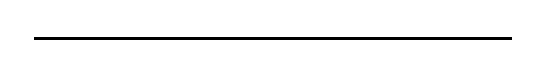
\begin{tikzpicture}
		\draw[thick, black] (0.25*\textwidth, 0) -- (0.75*\textwidth, 0);
		\node[rotate = 360 - 90, xshift = -0.6pt, yshift = 1pt] at (0.25*\textwidth,0){\decotwo};
		\node[rotate = 90, xshift = -0.6pt, yshift = 1pt] at (0.75*\textwidth,0){\decotwo};
	\end{tikzpicture}
	\end{center}
}

\pagestyle{fancy}

\newcommand{\lecday}[1][]
{
    \def\datee{#1}
    \fancyhead[L]{\datee}
}



\newcommand{\signature}
{
	\begin{tikzpicture}[remember picture,overlay]
		\node[fill = YellowOrange!20!white] at ([yshift = 1cm, xshift = -3cm]current page.south east) {\fontsize{10pt}{0pt}{\itshape Kara.$\mathcal{A}$}};
	\end{tikzpicture}
}

\AddToHook{shipout/background}{
  \begin{tikzpicture}[remember picture, overlay]
	  \node[] at ([yshift = 1.5cm,xshift = \textwidth /2 + 0.9cm]current page.south west) {\includegraphics[width = 0.5cm]{preview3}};
	  \node[] at ([yshift = 1.5cm,xshift = - \textwidth /2 - 0.9cm]current page.south east) {\includegraphics[width = 0.5cm]{preview4}};
  \end{tikzpicture}
}



\newtcolorbox[auto counter, number within = section]{remark}[1][]
{
       		title = Remark #1,
		enhanced,
		boxrule = 0pt,
		colback = white,
		breakable,
		arc = 4pt,
		colbacktitle = cyan,
		colback = cyan!5!white,
		segmentation style =
		{
			solid,cyan,thick,
		},
		attach boxed title to top left =
		{
			xshift = 0cm,
		},
		boxed title style =
		{
			boxrule = 0pt,
			sharp corners,
			drop fuzzy shadow = {cyan},
		},
		drop fuzzy shadow = {cyan!80!black},
}

\newtcolorbox[auto counter, number within = section]{theorem}[1][]
{                                      
		title = Theorem \thetcbcounter : #1,
		enhanced, 
		boxrule = 0pt,
		colback = white,
		breakable,
		arc = 4pt,
		colbacktitle = purple,
		colback = purple!5!white,
		segmentation style = 
		{
			solid, purple,thick,
		},
		attach boxed title to top left = 
		{
			xshift = 0cm, 
		},
		boxed title style = 
		{
			boxrule = 0pt,
			sharp corners,
			drop fuzzy shadow = {purple},
		},
		drop fuzzy shadow = {purple!80!black},
}

\newtcolorbox[auto counter, number within = section]{definition}[1][]
{                                      
		title = Definition \thetcbcounter : #1,
		enhanced, 
		boxrule = 0pt,
		colback = white,
		arc = 4pt,
		breakable,
		colbacktitle = YellowOrange!80!black,
		segmentation style = 
		{
			solid, YellowOrange,thick,
		},
		attach boxed title to top left = 
		{
			xshift = 0cm, 
		},
		colback = YellowOrange!5!white,
		boxed title style = 
		{
			boxrule = 0pt,
			sharp corners,
			drop fuzzy shadow = {YellowOrange!80!orange},
		},
		drop fuzzy shadow = {YellowOrange!80!black},
}

\newtcolorbox[auto counter, number within = section]{corollary}[1][]
{                                      
		title = corollary \thetcbcounter : #1,
		enhanced, 
		boxrule = 0pt,
		colback = white,
		arc = 4pt,
		breakable,
		colbacktitle = YellowOrange!80!black,
		segmentation style = 
		{
			solid, YellowOrange,thick,
		},
		attach boxed title to top left = 
		{
			xshift = 0cm, 
		},
		colback = YellowOrange!5!white,
		boxed title style = 
		{
			boxrule = 0pt,
			sharp corners,
			drop fuzzy shadow = {YellowOrange!80!orange},
		},
		drop fuzzy shadow = {YellowOrange!80!black},
}


\newtcolorbox{example}[1][]
{                                      
		title = Example,
		enhanced, 
		boxrule = 0pt,
		colback = white,
		arc = 4pt,
		segmentation style = 
		{
			solid, SpringGreen,thick,
		},
		breakable,
		colback = SpringGreen!5!white,
		colbacktitle = SpringGreen!80!black,
		attach boxed title to top left = 
		{
			xshift = 0cm, 
		},
		boxed title style = 
		{
			boxrule = 0pt,
			sharp corners,
			drop fuzzy shadow = {SpringGreen!80!orange},
		},
		drop fuzzy shadow = {SpringGreen!80!black},
}


\newcommand{\integral}[4]{\int\limits_{#1}^{#2} #4 d#3}
\newcommand{\limit}[3]{\lim\limits_{#1 \rightarrow #2} #3}
\newcommand{\strone}[2]{\left[ \begin{gathered}#1\\ #2\end{gathered} \right] }
\newcommand{\strtwo}[2]{\left\{ \begin{gathered}#1\\ #2\end{gathered} \right\} }
\newcommand{\strthree}[2]{\left\lfloor \begin{gathered}#1\\ #2\end{gathered} \right\rfloor }


\newcommand{\startbf}[1]{\text{\bfseries{#1}}}
\newcommand{\sett}[1]{\left\{ #1 \right\}}
\newcommand{\thesis}[1]{\left( #1 \right)}
\newcommand{\brkt}[1]{\left[ #1 \right]}
\newcommand{\floor}[1]{\left\lfloor #1 \right\rfloor}


\DeclareMathOperator{\img}{im} % Image
\DeclareMathOperator{\Img}{Im} % Image
\DeclareMathOperator{\coker}{coker} % Cokernel
\DeclareMathOperator{\Coker}{Coker} % Cokernel
\DeclareMathOperator{\Ker}{Ker} % Kernel
\DeclareMathOperator{\rank}{rank}
\DeclareMathOperator{\Spec}{Spec} % spectrum
\DeclareMathOperator{\Tr}{Tr} % trace
\DeclareMathOperator{\pr}{pr} % projection
\DeclareMathOperator{\ext}{ext} % extension
\DeclareMathOperator{\pred}{pred} % predecessor
\DeclareMathOperator{\dom}{dom} % domain
\DeclareMathOperator{\ran}{ran} % range
\DeclareMathOperator{\Hom}{Hom} % homomorphism
\DeclareMathOperator{\Mor}{Mor} % morphisms
\DeclareMathOperator{\End}{End} % endomorphism


\newcommand{\lm}{\ensuremath{\lambda}}
\newcommand{\eps}{\ensuremath{\epsilon}}
\newcommand{\veps}{\ensuremath{\varepsilon}}
\newcommand{\al}{\ensuremath{\alpha}}
\newcommand{\bb}{\ensuremath{\beta}}
\newcommand{\cc}{\ensuremath{\gamma}}
\newcommand{\dd}{\ensuremath{\delta}}
\newcommand{\DD}{\ensuremath{\Delta}}
\newcommand{\ff}{\ensuremath{\phi}}
\newcommand{\FF}{\ensuremath{\varphi}}

\newcommand{\RR}{\mathbb{R}}
\newcommand{\RO}{\mathcal{R}}
\newcommand{\EE}{\mathbb{E}}
\newcommand{\CC}{\mathbb{C}}
\newcommand{\RW}{\mathbb{R}^2}
\newcommand{\RT}{\mathbb{R}^3}
\newcommand{\RN}{\mathbb{R}^n}
\newcommand{\DS}{\mathcal{D}}

\newcommand{\KK}{\mathbb{K}}
\newcommand{\KW}{\mathbb{K}^2}
\newcommand{\KT}{\mathbb{K}^3}
\newcommand{\KN}{\mathbb{K}^n}

\newcommand{\NN}{\mathbb{N}}

\newcommand{\PS}{\mathcal{P}}
\newcommand{\AS}{\mathcal{E}}
\newcommand{\FS}{\mathcal{F}}
\newcommand{\LS}{\mathcal{L}}
\newcommand{\MS}{\mathcal{M}}


















\lecday[2025-03-18]

% \begin{document}

- \textbf{Problem :} \it (How to compute $e^{A} $ in general ?) 


- \textbf{The Solution :} \it \\
For $n \in \NN $ , and $A  \in \mathcal{M} _{n}(\KK) $, 
$\KK = \RR  $ or $\CC  $, to compute $e^{A} $, we use
the Dunford decomposition of $A$, we write $A$ as, 
\[
A = U + N  \quad  \left( U,N \in \mathcal{M} _{n}(\KK)  \right)
\]
with, 
\begin{itemize}
	\item $U$ is diagonalizable in other words
		there exist $P \in GL(\KK)   $  and 
		$D \in \mathcal{M} _{n}(\KK)  $  diagonal
		such that  $U = PDP ^{-1} $.
	\item  $N $ is nilpotent 
		$\text{ i.e. } $  there exist $k \in \NN $ 
		such that.
		$N^{k}= 0$ 
	\item $U $ commutes with $N $ $\text{ i.e. } UN = NU $.  
\end{itemize}
So, since $U $ and $N $ commute with $N $, we have 
\[
	e^{A} = e^{U+N} = e^{U} \cdot e^{N}
\]
but we have 
\[
e^{U} = e^{P D P ^{-1}} = P e^{D} P ^{-1}
\]
and \[
e^{N} = \sum_{l=0}^{\infty } = \frac{N^{l}}{l!} = 
\sum_{l=0}^{k-1} \frac{N^{l}}{l !}
\]

(since $N ^{l} = 0 $ for $l \geq k $), 
hence we obtain the closed form of $e^{A}$. 

Note that the Dunford decomposition of $A $ can be obtained
by using the jordan form $A$.
\divider
\it By the same way, we can define $\sin{(f) } $,
$\cos{(f) }$, $\sinh{(f) } $, etcetera, when $f $ is 
continuous, linear operator of a Banach space 
\[
\cos{(x) } = 
1 - \frac{x^2 }{2 !} + \frac{x^{4}}{4!} + \hdots 
\]
\divider
- \textbf{Exercise : } \it (Important)
Let $E $ be a Banach space, we denote by 
$\mathcal{G} \mathcal{L} (E)  $, the set of endomorphisms of
$g $ of $E $ which are continuous, invertible, and for which
$g^{-1} $ is continuous, we have 
\[
\mathcal{G} \mathcal{L} (E)  \subset \mathcal{L} (E) 
\]
\begin{enumerate}[(1)]
\item Let $f \in \mathcal{L} (E)  $ satisfying $\mid \mid \mid  f \mid \mid \mid  < 1$
\begin{enumerate}
\item Show that $\left( id_{E} + f \right) $ and 
	$\left( id_{E} - f \right) $  are in 
	in $\mathcal{G} \mathcal{L} (E)  $ 
\end{enumerate}
\item Deduce that $\mathcal{G} \mathcal{L}(E)   $  is an open
	subset of $\mathcal{L} (E)  $ 
\item Show that the map 
	\[
	\begin{array}{cccc}
	        & \mathcal{G}\mathcal{L}(E)       & \longrightarrow
		^{\ff}& \mathcal{G}\mathcal{L}(E)    \\
		      & f  \rightarrow & f^{-1}
	\end{array}
	\]
	is continuous 
\end{enumerate}
- \textbf{Solution :  }   

\begin{enumerate}[(1)]
\item  First, the continuity and the 
       linearity of $\left( id_{E} + f \right) $  
       and $\left( id_{E} - f \right) $ are obvious, 
       are obvious next consider the series 
       \[
	       \sum_{n=0}^{\infty}  f^{n}  
	       \quad \text{ of }  \quad 
	       \mathcal{L} \left( E \right) 
	       \text{ We have } 
       \]
       for all $n \in \NN_{0} $,
       \[
       \mid \mid \mid  f^n  \mid \mid \mid  \quad 
       \leq \quad  \mid \mid \mid  f \mid \mid \mid ^n 
       \]
       Since $\mid \mid \mid  f \mid \mid \mid  <  1 $ then
       the real geoemetric series 
       $\sum_{n=0}^{\infty}  \mid \mid \mid  f \mid \mid \mid ^n  $ 
       is convergent, thus 
       the real series $\sum_{n=0}^{\infty}  
       \mid \mid \mid  f^n  \mid \mid \mid $ 
       is also convergence, in other words the series
       $\sum_{n=0}^{\infty}  f^n  $  of $\mathcal{L} (E)  $ 
       is normally convergent, since 
       $\mathcal{L} (E)  $ is Banach because $E $ is banach,
       then $\sum_{n=0}^{\infty}  f^n  $ is convergent 
       in $\mathcal{L}(E)$, set 
       \[
       g = \sum_{n=0}^{\infty}  f^n \in  \mathcal{L} (E)  
       \]
       we have for all $n \in \NN_0$,
       \[
       \left( id_{E} - f \right) \circ 
       \sum_{n=0}^{N} 
       f^n  = 
       \sum_{n=0}^{N} \left( f^n - f^{n+1} \right) =
       id_{E} - f^{N+1}
       \]
       By letting $N \rightarrow \infty  $, we get, 
       \[
       \left( id_{E} - f \right) \circ 
       g = id_{E} 
       \]
       we prove by the same way that 
       $g \circ  \left( id_{E}-f \right)  = id_{E}$, 
       thus $\left( id_{E} - f \right) $ is invertible 
       and $\left( id_{E} - f \right)^{-1} = g =
       \sum_{n=0}^{\infty }f^n \in \mathcal{L} (E)$, thus, 
       \[
       \left( id_{E} -f  \right) \in 
       \mathcal{G} \mathcal{L} (E)  
       \]
       \divider
       \it (motivation $(1-x) \times \frac{1}{1-x}  = 1 $ )
       \divider
       by replacing $f $ by $-f$, we find that 
       $\left( id_{E} + f \right) $ is also invertible is also
       invertible and 
       \[
       \left( id_{E} + f \right)^{-1}=
       \sum_{n=0}^{\infty}  (-f) ^n = 
       \sum_{n=0}^{\infty}  (-1) ^n f^n 
       \in  \mathcal{L} (E) 
       \]
       Consequently $\left( id_{E} + f \right) \in \mathcal{G} 
       \mathcal{L} (E)$  
     \item 
	     \begin{center}
	     	\it $\mathcal{G} \mathcal{L} (E)  $ is 
		an open subset of $\mathcal{L} (E)  $ ??
	     \end{center}
	     \normalfont
	     we have to show that $\mathcal{G} \mathcal{L} 
	     (E) $  is a neighborhood of all if elements 
	     so, let 
	     $f_0 \in \mathcal{G} \mathcal{L} (E) $ arbitrary
	     and let us show that $\exists r  > 0 $ such that
	     $\mathcal{B} _{\mathcal{L} (E) }
	     (f_0, \frac{1}{\mid \mid \mid  f_0 ^{-1}\mid \mid \mid }) 
	     $.
	     \begin{center}
		     That is 
		     $f \in  \mathcal{L} (E)  $  
		     and $
		     \mid \mid \mid  f-f_0 \mid \mid \mid 
		     < \frac{1}{\mid \mid \mid  f_0^{-1} \mid \mid \mid }$ 
	     \end{center}
	     let us show that $f \in  \mathcal{G}
	     \mathcal{L} (E) $, we have 
	     \begin{align*}
		     \mid \mid \mid  
		     f_0^{-1}
		     \circ f - id_{E}\mid \mid \mid  
		     = 
		     \mid \mid \mid  f_0^{-1}
		     \circ \left( f-f_0 \right)\mid \mid \mid &
		     \leq \mid \mid \mid  f_0^{-1} \mid \mid \mid  
		     \cdot 
		     \underbrace{
		     \mid \mid \mid  f-f_0 \mid \mid \mid 
		     }_{< \frac{1}{\mid \mid \mid  f_0^{-1} \mid \mid \mid }} 
							   \\ &< 1
	     \end{align*}
	     thus according to the result of Question $(1)$, we have
	     \[
	     \left( f_0^{-1} \circ 
	     f - id_{E}\right) 
	     + id_{E} = f_0^{-1} \circ  f \in 
	     \mathcal{G} \mathcal{L} (E) 
	     \]
	     Thus, 
	     \[
	     f = f_0 \circ 
	     \left( f_0 ^{-1} \circ  f \right) 
	     \in \mathcal{G} \mathcal{L} (E) 
	     \]
	     as required, this confirms the inclusion, 
	     so $\mathcal{G} \mathcal{L} (E)  $  is 
	     a neighborhood of any $f_0 \in 
	     \mathcal{G} \mathcal{L} (E) $, so $\mathcal{G} 
	     \mathcal{L} (E) $ is an open subset of $\mathcal{L} 
	     (E)$.
	     \begin{align*}
	     \mathcal{G} 
	     \mathcal{L} (\RR ^n )  
	     &= GL(\RR ^n ) \simeq 
	     GL_{n}(\RR )  \\
	     &= 
	     \left\{ A \in  \mathcal{M} _{n}(\RR ) :
	     det(A) \neq  0\right\} \\
	     &= \left\{ A \in  \mathcal{M} _{n}(\RR ) : 
	     det(A) \in (-\infty ,0) \cup (0,\infty ) \right\} \\
	     &= det^{-1}((-\infty , 0) \cup (0,\infty ) )  
	     \end{align*}
	     \item 
		     \[
		     \begin{array}{cccc}
		             &  \mathcal{G} 
			      \mathcal{L} (E) & \longrightarrow^{\ff }& 
			      \mathcal{G} \mathcal{L} (E) \\
		                &  f  & \longmapsto     & f^{-1} \\ 
		     \end{array}
		     \]
		     is continiuous ??, let us show 
		     the continuity  of 
		     $\ff  $ at some $f_0 \in 
		     \mathcal{G} \mathcal{L} (E) $
		     arbitrary, for all $f \in  
		     \mathcal{G} \mathcal{L} (E) $, such that
		     \[
		     \mid \mid \mid  f-f_0 \mid \mid \mid  
		     < 
		     \frac{1}{\mid \mid \mid  f_0^{-1} \mid \mid \mid }
		     \]
		     we have,
		     \begin{align*}
			     f^{-1}-f_0^{-1} &=
			     f_0^{-1} \circ 
			     \left( f_0 \circ  f^{-1}
			     - id_{E}\right) \\
					     &= 
					     f_0^{-1} \circ 
					     \left( 
					    f_0
				    \circ f^{-1} - id_{E}\right) 
				    \\
					     &=
		f_0^{-1} \circ 
		\left( \left( f \circ f_0^{-1} \right)
		^{-1} - id_{E}\right) \\
					     &=
		f_0^{-1} \circ 
		\left( 
			\left( f-f_0+f_0 \right)
			\circ f_0^{-1}
		\right)^{-1} - id_{E} \\
					     &= f_0^{-1}
					\circ 
	\left[ 
		\left( 
			\left( 
				f-f_0
			\right) \circ 
			f_0^{-1} + id_{E}
		\right)^{-1} 
		-id_{E}
	\right]
		     \end{align*}
		     From Question $(1)$, 
		     \begin{align*}
		     f_0^{-1}
		     \circ 
		     \left[ 
			     \sum_{n=0}^{\infty}  
			   (-1) ^n 
			   \left( 
				   \left( f-f_0 \right)
				   \circ f_0^{-1}
			   \right)^n -id_{E}
		     \right]
		     \end{align*}
		     Hence 
		     \begin{align*}
		     \mid \mid \mid  f^{-1}
		     - f_0^{-1}\mid \mid \mid  
		     \leq 
		     \mid \mid \mid  f_0^{-1} \mid \mid \mid  
		    \sum_{n=0}^{\infty}  
		    \mid \mid \mid  (-1) ^n 
		    \left( 
			    \left( f-f_0 \right)
			    \circ f_0^{-1}
		    \right)^n 
		    \mid \mid \mid 
		     \end{align*} 
		     Hence 
		     \begin{align*}
		     \mid \mid \mid  f^{-1}
		     -f_0^{-1}\mid \mid \mid  
		     & \leq 
		     \mid \mid \mid  f_0^{-1} \mid \mid \mid  
		    \sum_{n=1}^{\infty}  
		    \mid \mid \mid  (-1) ^n 
		    ((f-f_0) \circ  f_0^{-1}) ^n 
		    \mid \mid \mid  \\
		    & \leq       \mid \mid \mid  
		    f_0^{-1}\mid \mid \mid 
		    \cdot 
		    \sum_{n=0}^{\infty}  
		    \mid \mid \mid  f-f_0 \mid \mid \mid ^n 
		    \mid \mid \mid  f_0^{-1} \mid \mid \mid ^n 
		    \end{align*} 
		    Thus,
		    \[
		    \mid \mid \mid  f^{-1}
		    -f_0^{-1}\mid \mid \mid  
		    \leq \mid \mid \mid  f_0^{-1} \mid \mid \mid  
		    \cdot 
		    \left[ 
			    \frac{\mid \mid \mid  f-f_0 \mid \mid \mid 
			    \cdot \mid \mid \mid  f_0^{-1} \mid \mid \mid }{
		    1 - \mid \mid \mid  f-f_0 \mid \mid \mid 
	    \cdot \mid \mid \mid  f_0^{-1} \mid \mid \mid }
		    \right]
		    \]
		    This shows that, 
		    \[
			    \lim_{f \to f_0} 
			    \mid \mid \mid  
			    f^{-1} - f_0^{-1}
			    \mid \mid \mid  =
			    0
		    \]
		    That is 
		    $f^{-1} \rightarrow f_0^{-1}$,
		    $f \rightarrow f_0$, hence consequently
		    $\ff  $ is continiuous 
\end{enumerate}
\begin{definition}[]
Let $E $ be a N.V.S, A series 
$\sum_{n=1}^{\infty} x_{n}   $ 
of $E $ is said to be  unconditionally convergent
if for every permutation 
$ \sigma    : \NN \longrightarrow \NN$, the series
$\sum_{n=0}^{\infty}  x_{ \sigma (n)   } $ converges to 
 the same sum (in particular, the series $\sum_{n=0}^{\infty}  x_{n} $ 
converges).
\end{definition}

% \end{document}













